% GNUPLOT: LaTeX picture with Postscript
\begingroup
  \makeatletter
  \providecommand\color[2][]{%
    \GenericError{(gnuplot) \space\space\space\@spaces}{%
      Package color not loaded in conjunction with
      terminal option `colourtext'%
    }{See the gnuplot documentation for explanation.%
    }{Either use 'blacktext' in gnuplot or load the package
      color.sty in LaTeX.}%
    \renewcommand\color[2][]{}%
  }%
  \providecommand\includegraphics[2][]{%
    \GenericError{(gnuplot) \space\space\space\@spaces}{%
      Package graphicx or graphics not loaded%
    }{See the gnuplot documentation for explanation.%
    }{The gnuplot epslatex terminal needs graphicx.sty or graphics.sty.}%
    \renewcommand\includegraphics[2][]{}%
  }%
  \providecommand\rotatebox[2]{#2}%
  \@ifundefined{ifGPcolor}{%
    \newif\ifGPcolor
    \GPcolortrue
  }{}%
  \@ifundefined{ifGPblacktext}{%
    \newif\ifGPblacktext
    \GPblacktextfalse
  }{}%
  % define a \g@addto@macro without @ in the name:
  \let\gplgaddtomacro\g@addto@macro
  % define empty templates for all commands taking text:
  \gdef\gplbacktext{}%
  \gdef\gplfronttext{}%
  \makeatother
  \ifGPblacktext
    % no textcolor at all
    \def\colorrgb#1{}%
    \def\colorgray#1{}%
  \else
    % gray or color?
    \ifGPcolor
      \def\colorrgb#1{\color[rgb]{#1}}%
      \def\colorgray#1{\color[gray]{#1}}%
      \expandafter\def\csname LTw\endcsname{\color{white}}%
      \expandafter\def\csname LTb\endcsname{\color{black}}%
      \expandafter\def\csname LTa\endcsname{\color{black}}%
      \expandafter\def\csname LT0\endcsname{\color[rgb]{1,0,0}}%
      \expandafter\def\csname LT1\endcsname{\color[rgb]{0,1,0}}%
      \expandafter\def\csname LT2\endcsname{\color[rgb]{0,0,1}}%
      \expandafter\def\csname LT3\endcsname{\color[rgb]{1,0,1}}%
      \expandafter\def\csname LT4\endcsname{\color[rgb]{0,1,1}}%
      \expandafter\def\csname LT5\endcsname{\color[rgb]{1,1,0}}%
      \expandafter\def\csname LT6\endcsname{\color[rgb]{0,0,0}}%
      \expandafter\def\csname LT7\endcsname{\color[rgb]{1,0.3,0}}%
      \expandafter\def\csname LT8\endcsname{\color[rgb]{0.5,0.5,0.5}}%
    \else
      % gray
      \def\colorrgb#1{\color{black}}%
      \def\colorgray#1{\color[gray]{#1}}%
      \expandafter\def\csname LTw\endcsname{\color{white}}%
      \expandafter\def\csname LTb\endcsname{\color{black}}%
      \expandafter\def\csname LTa\endcsname{\color{black}}%
      \expandafter\def\csname LT0\endcsname{\color{black}}%
      \expandafter\def\csname LT1\endcsname{\color{black}}%
      \expandafter\def\csname LT2\endcsname{\color{black}}%
      \expandafter\def\csname LT3\endcsname{\color{black}}%
      \expandafter\def\csname LT4\endcsname{\color{black}}%
      \expandafter\def\csname LT5\endcsname{\color{black}}%
      \expandafter\def\csname LT6\endcsname{\color{black}}%
      \expandafter\def\csname LT7\endcsname{\color{black}}%
      \expandafter\def\csname LT8\endcsname{\color{black}}%
    \fi
  \fi
  \setlength{\unitlength}{0.0500bp}%
  \begin{picture}(9636.00,10204.00)%
    \gplgaddtomacro\gplbacktext{%
    }%
    \gplgaddtomacro\gplfronttext{%
      \colorrgb{0.50,0.50,0.50}%
      \put(964,9948){\makebox(0,0){\strut{}$N_{\mathrm{NSHT}} = 23$}}%
      \put(4082,10203){\makebox(0,0){\strut{}Modal Beamformer}}%
      \put(964,7724){\makebox(0,0){\strut{}$\bar\mu_\phi = 0.12^\circ$}}%
    }%
    \gplgaddtomacro\gplbacktext{%
    }%
    \gplgaddtomacro\gplfronttext{%
      \colorrgb{0.50,0.50,0.50}%
      \put(2891,9948){\makebox(0,0){\strut{}$N_{\mathrm{NSHT}} = 10$}}%
      \put(2891,7724){\makebox(0,0){\strut{}$\bar\mu_\phi = 0.48^\circ$}}%
    }%
    \gplgaddtomacro\gplbacktext{%
    }%
    \gplgaddtomacro\gplfronttext{%
      \colorrgb{0.50,0.50,0.50}%
      \put(4818,9948){\makebox(0,0){\strut{}$N_{\mathrm{NSHT}} = 5$}}%
      \put(4818,7724){\makebox(0,0){\strut{}$\bar\mu_\phi = 2.50^\circ$}}%
    }%
    \gplgaddtomacro\gplbacktext{%
    }%
    \gplgaddtomacro\gplfronttext{%
      \colorrgb{0.50,0.50,0.50}%
      \put(6745,9948){\makebox(0,0){\strut{}$N_{\mathrm{NSHT}} = 3$}}%
      \put(6745,7724){\makebox(0,0){\strut{}$\bar\mu_\phi = 7.56^\circ$}}%
    }%
    \gplgaddtomacro\gplbacktext{%
    }%
    \gplgaddtomacro\gplfronttext{%
      \colorrgb{0.50,0.50,0.50}%
      \put(8672,10203){\makebox(0,0){\strut{}DSB}}%
      \put(8672,7724){\makebox(0,0){\strut{}$\bar\mu_\phi = 6.47^\circ$}}%
    }%
    \gplgaddtomacro\gplbacktext{%
    }%
    \gplgaddtomacro\gplfronttext{%
      \colorrgb{0.50,0.50,0.50}%
      \put(964,5173){\makebox(0,0){\strut{}$\bar\mu_\phi = 0.50^\circ$}}%
    }%
    \gplgaddtomacro\gplbacktext{%
    }%
    \gplgaddtomacro\gplfronttext{%
      \colorrgb{0.50,0.50,0.50}%
      \put(2891,5173){\makebox(0,0){\strut{}$\bar\mu_\phi = 1.16^\circ$}}%
    }%
    \gplgaddtomacro\gplbacktext{%
    }%
    \gplgaddtomacro\gplfronttext{%
      \colorrgb{0.50,0.50,0.50}%
      \put(4818,5173){\makebox(0,0){\strut{}$\bar\mu_\phi = 9.02^\circ$}}%
    }%
    \gplgaddtomacro\gplbacktext{%
    }%
    \gplgaddtomacro\gplfronttext{%
      \colorrgb{0.50,0.50,0.50}%
      \put(6745,5173){\makebox(0,0){\strut{}$\bar\mu_\phi = 19.99^\circ$}}%
    }%
    \gplgaddtomacro\gplbacktext{%
    }%
    \gplgaddtomacro\gplfronttext{%
      \colorrgb{0.50,0.50,0.50}%
      \put(8672,5173){\makebox(0,0){\strut{}$\bar\mu_\phi = 7.17^\circ$}}%
    }%
    \gplgaddtomacro\gplbacktext{%
    }%
    \gplgaddtomacro\gplfronttext{%
      \colorrgb{0.50,0.50,0.50}%
      \put(964,2622){\makebox(0,0){\strut{}$\bar\mu_\phi = 2.19^\circ$}}%
    }%
    \gplgaddtomacro\gplbacktext{%
    }%
    \gplgaddtomacro\gplfronttext{%
      \colorrgb{0.50,0.50,0.50}%
      \put(2891,2622){\makebox(0,0){\strut{}$\bar\mu_\phi = 3.03^\circ$}}%
    }%
    \gplgaddtomacro\gplbacktext{%
    }%
    \gplgaddtomacro\gplfronttext{%
      \colorrgb{0.50,0.50,0.50}%
      \put(4818,2622){\makebox(0,0){\strut{}$\bar\mu_\phi = 10.95^\circ$}}%
    }%
    \gplgaddtomacro\gplbacktext{%
    }%
    \gplgaddtomacro\gplfronttext{%
      \colorrgb{0.50,0.50,0.50}%
      \put(6745,2622){\makebox(0,0){\strut{}$\bar\mu_\phi = 13.75^\circ$}}%
    }%
    \gplgaddtomacro\gplbacktext{%
    }%
    \gplgaddtomacro\gplfronttext{%
      \colorrgb{0.50,0.50,0.50}%
      \put(8672,2622){\makebox(0,0){\strut{}}}%
    }%
    \gplgaddtomacro\gplbacktext{%
    }%
    \gplgaddtomacro\gplfronttext{%
      \colorrgb{0.50,0.50,0.50}%
      \put(964,71){\makebox(0,0){\strut{}$\bar\mu_\phi = 3.63^\circ$}}%
    }%
    \gplgaddtomacro\gplbacktext{%
    }%
    \gplgaddtomacro\gplfronttext{%
      \colorrgb{0.50,0.50,0.50}%
      \put(2891,71){\makebox(0,0){\strut{}$\bar\mu_\phi = 3.94^\circ$}}%
    }%
    \gplgaddtomacro\gplbacktext{%
    }%
    \gplgaddtomacro\gplfronttext{%
      \colorrgb{0.50,0.50,0.50}%
      \put(4818,71){\makebox(0,0){\strut{}$\bar\mu_\phi = 10.22^\circ$}}%
    }%
    \gplgaddtomacro\gplbacktext{%
    }%
    \gplgaddtomacro\gplfronttext{%
      \colorrgb{0.50,0.50,0.50}%
      \put(6745,71){\makebox(0,0){\strut{}$\bar\mu_\phi = 19.26^\circ$}}%
    }%
    \gplgaddtomacro\gplbacktext{%
    }%
    \gplgaddtomacro\gplfronttext{%
      \colorrgb{0.50,0.50,0.50}%
      \put(8672,71){\makebox(0,0){\strut{}}}%
    }%
    \gplbacktext
    \put(0,0){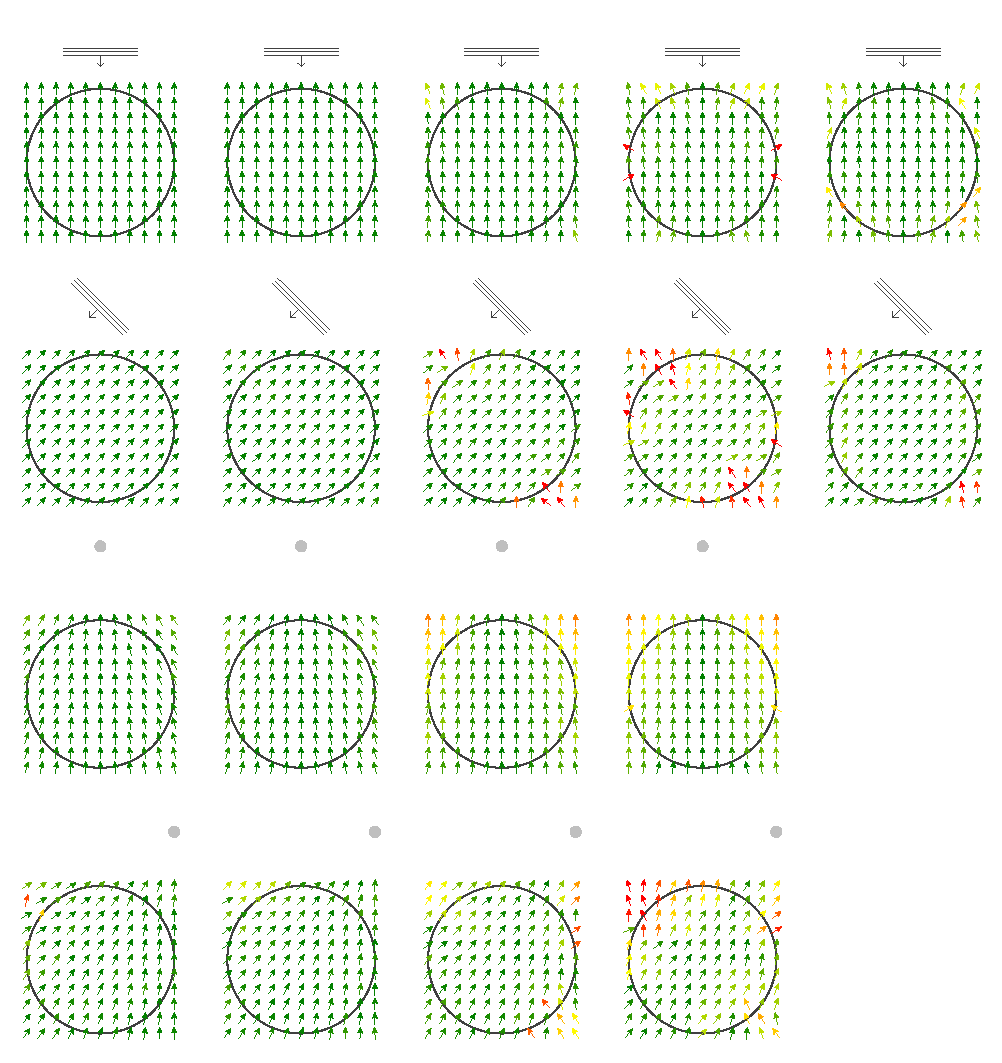
\includegraphics{fig}}%
    \gplfronttext
  \end{picture}%
\endgroup
